
%%% Local Variables: 
%%% mode: latex
%%% TeX-master: "main"
%%% End: 
\section{Exploratory Tools}
% This section should first describe why an exploratory tool was needed. Second, why was an interactive tool needed? Be brief.

As described in the previous section, inspection and description of the background signal was required to identify the previously mentioned misassemblies. Such illustration is typically accomplished with a genome browser. Genome browsers allow the exploration of sequencing datasets in high detail, producing publication-ready images of depth, coverage, features, and more. To facilitate this exploration, flexibility was a key aspect for selecting a genome browser for both identification and correction of assembly errors.

Specifically, an ideal genome browser would display depth, coverage, and annotation data from both strands separately. Visualization of multiple coverage vectors (e.g. different conditions) in a single track has improved data density compared to multi-track browser designs. Unfortunately, ``reducer'' functions (max, sum, average) are not simple to compute for multiple large alignment files and existing genome browsers. In fact, many conventional browsers are sluggish to even load such large datasets.\cite{191,192} These genome browsers did not meet the requirements for this project. Instead, a customized genome browser was constructed with flexibility, speed, and simplicity in mind to facilitate assembly visualization and curation with the sequencing data and genome annotations.

\begin{wrapfigure}{R}{0.4\textwidth}
\small
\vspace{-20pt}
\begin{center}
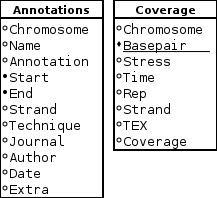
\includegraphics[width=0.38\textwidth]{images/Assembly/Browser/Genome_browser_schema.png}
\end{center}
\vspace{-20pt}
\caption{Database Tables}\label{fig:5.5}
A simple database was designed, indexing the annotations and coverage entities on their genomic coordinates.
\end{wrapfigure}

\subsubsection{Genome Browser}
In this genome browser, only the coverage vector was required for visualization and not the inspection of individual reads. A total of 169 gigabytes of aligned reads were summarized by 6.8 gigabytes of coverage vectors, a dramatic reduction of resource requirements. Still, these data were too large to transmit to users or perform reducing functions upon. The appropriate format for visualization and distribution of these data to the \textit{Clostridia} research community was a web application with a database. The objective for this genome browser was simple: allow users to upload and view feature annotations (e.g. sRNAs, proteins) alongside condition-specific coverage vectors from this sequencing dataset. The details of its construction have been described in the Methods chapter (\ref{app:browser_ui}).

The finished product was a modern genome browser with an intuitive user interface(\ref{app:browser_ui}). A simple database was required to host coverage and annotation records. An object relational model was required to retrieve and pass data to the web application layer for conversion into scalable vector graphics (SVG). This creation had both speed, with optimized SQL queries, and flexibility, with interactive zooming, filtering, and tooltip details. Strand specific coverage and annotations were displayed in a publication ready form. This genome browser was a tool to integrate annotation types including the transcriptome assembly, reference CDSes, and more, contextualizing these genomic features with expression data. After construction, this genome browser was loaded with genome annotations to facilitate error correction.

\subsubsection{Promoter Prediction Tool}
To aid the curation process, it was desirable to integrate additional annotations such as promoter and terminator predictions. For example, promoter predictions help resolve misassembly near transcription start sites. Promoter motifs are genomic signals that should correlate with expression levels at a rate predictable from sequence similarity to a consensus motif. Unfortunately, promoter annotations do not exist for \textit{C. acetobutylicum}. After observing the extended transcripts and UTRs in the previous section, a promoter prediction tool was developed to address these errors.

A promoter prediction tool was developed to utilize consensus sequences from \textit{B. subtilis}\cite{189} to predict promoter motifs in this \textit{C. acetobutylicum}. The promoter prediction tool, described in \ref{methods:promoter_prediction}, converts consensus sequences into models suitable for input into the MAST algorithm.\cite{5} Consensus sequences from DBTBS\cite{189} were used to generate models of promoter elements and transcription factor binding sites. Then, these were used to scan the \textit{C. acetobutylicum} genome. Predictions with p \textless 0.01 were then converted to GTF format and uploaded into the browser. This browser, loaded with annotations, was then used to visualize errors in the uncurated assembly and discussed in the next section.

These exploratory tools were created to improve the precision of the transcript boundary estimates by contextualizing the coverage patterns with annotations (e.g. Rho-independent terminators, promoters motifs) that explain drops in depth. These genomic signals provide biological mechanisms for the depth and coverage observations, increasing the amount of useful signals present at transcript boundaries. These annotations were combined in a customized genome browser to be used for integrative analyses of these genomic signals and sequencing data. 




